\chapter{Background}
This chapter covers the different topics that are present in this thesis.
The background starts by briefly covering Chip Multicore Processors and Heterogeneous Chip Multicore Processors to motivate the existence and research conducted in Dynamic Multicore Processors (DMP).
This is followed by a description of the three types of Dynamic Multicore Processors that currently exists.
Then the Explicit Data Graph Execution (EDGE) instruction set architecture (ISA) is described; this is the ISA used by the DMP explored throughout this thesis.
Specific features of an EDGE Processor, including the ability to fuse cores is then explained in detail.
Finally, streaming programming languages, which are used in Chapter~ref{}, and the different machine learning techniques utilised in the thesis are explained.

\section{Chip Multicore Processors}

\begin{figure}[t]
 \center
 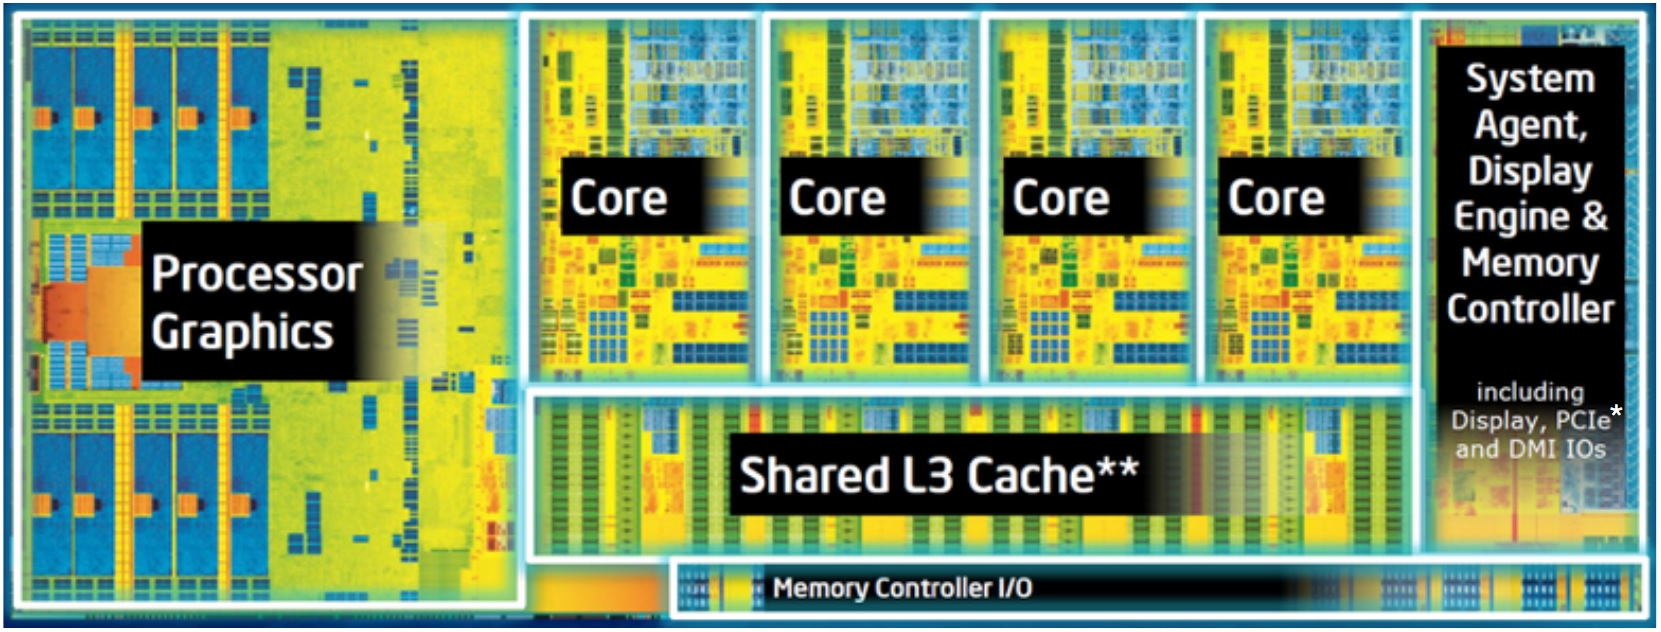
\includegraphics[width=1\textwidth]{background/graphics/i7intel.jpg}
 \caption{Intel Core i7 processor internal die photograph taken from intel whitepaper}\label{fig:i7}
\end{figure}
 
Chip Multicore Processors (CMPs) have become ubiquitous due to the difficulty in scaling single core performance.
In a CMP, multiple processor cores are put on a single package as can be seen in Figure~\ref{fig:i7}.
The most common CMP uses homogeneous cores as they reduce the design complexity both from a hardware and software perspective~\cite{}.
Unlike single core systems, the performance improvement in CMPs come from running multiple tasks in parallel.
These tasks can either be different programs or multiple threads from the same program running on the multiple cores.
By defining speedup \textit{S} to be the original execution time of the program over the new execution time with \textit{n} processors and \textit{f} representing the fraction of the program which can be parallelised; Amdahl's Law states

\begin{equation}
S = \frac{1}{(1-f) + \frac{f}{n}}
\end{equation}\label{amdlaw}

thus, given an infinite number of processor cores~\cite{ekhout2010amdalh}

\begin{equation}
\lim_{n\to\infty} S = \frac{1}{(1-f)}
\end{equation}

This second equation demonstrates how, given any program, the speedup obtained by using a CMP will be limited to the fraction \textit{f} of parallel code found in the program itself.
As all the processor cores are homogeneous t	his will cause serial bottlenecks to severely reduce the potential speedup as no core is adapted to speedup such regions.
This implication has pushed research into finding ways of parallelising code to its fullest~\cite{}, however this may not always be possible~\cite{}.
Thus whilst CMPs have become a mainstain in processor design, the homogeneous model has its limits.

\section{Heterogeneous Chip Multicore Processors}

\begin{figure}[t]
 \center
 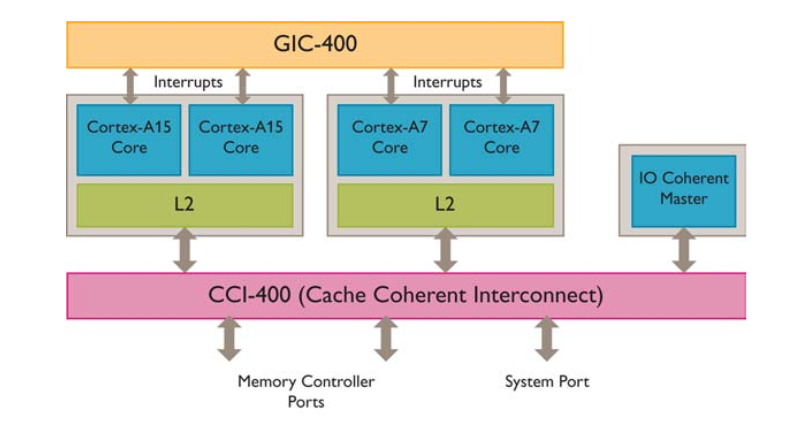
\includegraphics[width=1\textwidth]{background/graphics/biglittle.png}
 \caption{Example of a heterogeneous multicore processor proposed by ARM (big.LITTLE)}\label{fig:blarm}
\end{figure}

Unlike CMPs, Heterogeneous Chip Multicore Processors (HCMPs) or Asymmetrical Chip Multicore Processors (ACMPs) bring a variety of cores onto a single package.
This may come in different forms, such as having multiple instruction set architectures on the same system on chip (MPSoCs)~\cite{venkat2014harnessingisa,venkatHipstr2016}, or same ISA different size cores on an SoC~\cite{bigLittle}.
For example, Figure~\ref{fig:blarm} shows a schemata for ARM's big.LITTLE HCMP, where a high-performance Cortex-A15 is paired with a simpler, power efficient Cortex-A7.
The two cores are connected via a cache coherent interconnect which provides data coherence at the bus-level, allowing the cores to make reads to its neighbor.
Software is then run on one of the cores depending on a profile; if the user requires performance over energy, then the Cortex-A15 will be chosen, however if energy/power efficiency is required then the Cortex-A7 will be chosen.

This small example already demonstrates an advantage of HCMPs; unlike CMPs, the variety of cores on an HCMP provide a flexibility to the hardware.
This can be used for different purposes, such as security~\cite{venkatHipstr2016}, energy/power savings~\cite{venkat2014harnessingisa} and speeding up applications~\cite{venkat2014harnessingisa}.
In their 2014 paper, Venkat et al.~\cite{venkat2014harnessingisa} demonstrate that a multi-ISA HCMP can improve performance by up to 1.4x and achieve energy savings of up to 40\% compared to a CMP on a peak-power budget of 40W.
They motivate the idea that HCMPs with heterogeneous ISAs even improve over the performance of single-ISA HCMPs with speedups around 15\% and energy savings of 21.5\%.

However, whilst the hardware diversity in HCMPs is an advantage compared to CMPs, it also increases programming complexity.
For example, Gupta et al. in ~\cite{Gupta2017Dypo} show that a single-ISA octa-core big.LITTLE architecture can have 20 CPU cores, combined with the ability to dynamically modify the voltage, this leads to 4000 different configurations.
This highly increases the complexity of obtaining the correct settings for different programs.
MPSoCs also face a similar issue as having more than a single ISA not only adds design challenges, but program migration between different cores may in fact deteriorate performance~\cite{DeVuystMigration2012}.

\section{Dynamic Multicore Processors}

% This section explains what a dynamic multicore is

In both CMPs and HCMPs, once the chip is fabricated the design cannot be modified, meaning that many of the trade-offs between power, performance and area cannot be changed after production.
Dynamic Multicore Processors (DMPs) attempt to bridge the gap between the two previous designs by allowing the execution substrate to adapt dynamically at runtime.
Mitall's survey ~\cite{MittalSurv2016} defines three types of modifiable resources: the core count~\cite{ipek2007CoreFusion}, number of resources that each core has~\cite{Homayoun3DPooling2012} and microarchitectural features~\cite{fallinhetblock2014,BauerRSE08,tavanaElastic}.

\subsection{Core Fusion Dynamic Multicore Processors}

\begin{figure}[t]
    \centering
    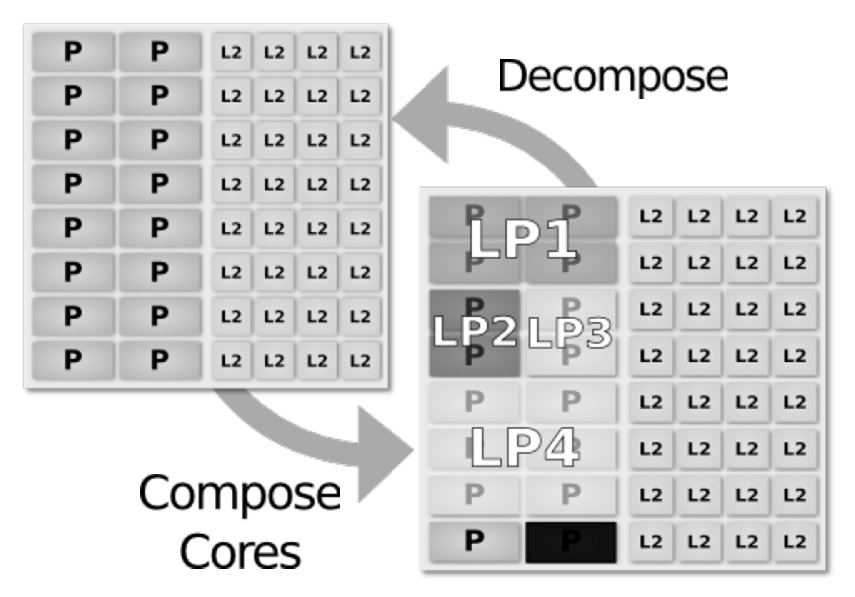
\includegraphics[width=.7\textwidth]{streamit-paper/graphics/dmcgraph.pdf}
    \caption{High-level view of a dynamic multicore processor that can modify its core count.}
    \label{fig:dynmulticore}
\end{figure}

A DMP that modifies core count is composed of homogeneous cores with a reconfigurable fabric.
Physical cores can function either on their own or as a group of physical cores; this is called a Logical Core (LC).
Throughout this thesis, the term core-fusion will be used to define the mechanism of cores creating an LC.
A logical core will fetch instructions from a single source and execute them accross all the physical cores that compose the LC.
Cores can fuse dynamically and create a logical core of any sizes.
For example in Figure~\ref{fig:dynmulticore}, the DMP fuses cores into 3 LCs of sizes 1, 8 and 6 physical cores.
The exact mechanism of core-fusion are described later on in Section~\ref{sec}.

The advantage of a core-fusion DMP over the traditional CMP or HCMP is the ability to reconfigure the processor dynamically to better match the tasks at hand.
For example, large sequential sections of code with high Instruction Level Parallelism (ILP) can be accelerated on a logical core that mimics a wide superscalar processor.
On parallel workloads the DMP can be reconfigured by de-composing the logical cores as seen in Figure~\ref{fig:dynmulticore} to match the Thread Level Parallelism (TLP).

%More here
\subsection{Resource Sharing Dynamic Multicore Processors}
A more fine-grained reconfiguration can be found in resource-sharing DMPs.
There exist different models for resource sharing DMPs.
For example the WiDGET DMP by Watanabe et al.~\cite{Watanabe2010Widget}, cores are built out of Instruction Engine front-ends which function similarly to Out of Order (OoO) cores' front and back ends.
They then are connected to Execution Units which they can choose to use.
Each core in the WiDGET DMP also have access to their neighbors Execution Units, allowing for more variation.
Another example of resource sharing can be found in Rodrigues et al.'s work~\cite{rodrigues2014perf} where a core can use resources such as Arithmetic Logic Units (ALUs) from other cores.

%More here
\subsection{Microarchitectural Reconfigurable Dynamic Multicore Processors}
A final example is a DMP which can reconfigure microarchitectural features to better fit the current application.
Fallin et al.~\cite{fallin} observe that serial code can exhibit phases that fit different microarchitectural features.
According to them, these phases may only been in the ten to hundred thousands instructions long.
These DMPs can therefore modify microarchitecural features, such as in-order or out-of-order execution, to best match the current phase of a program.

\begin{figure}[t]
    \centering
    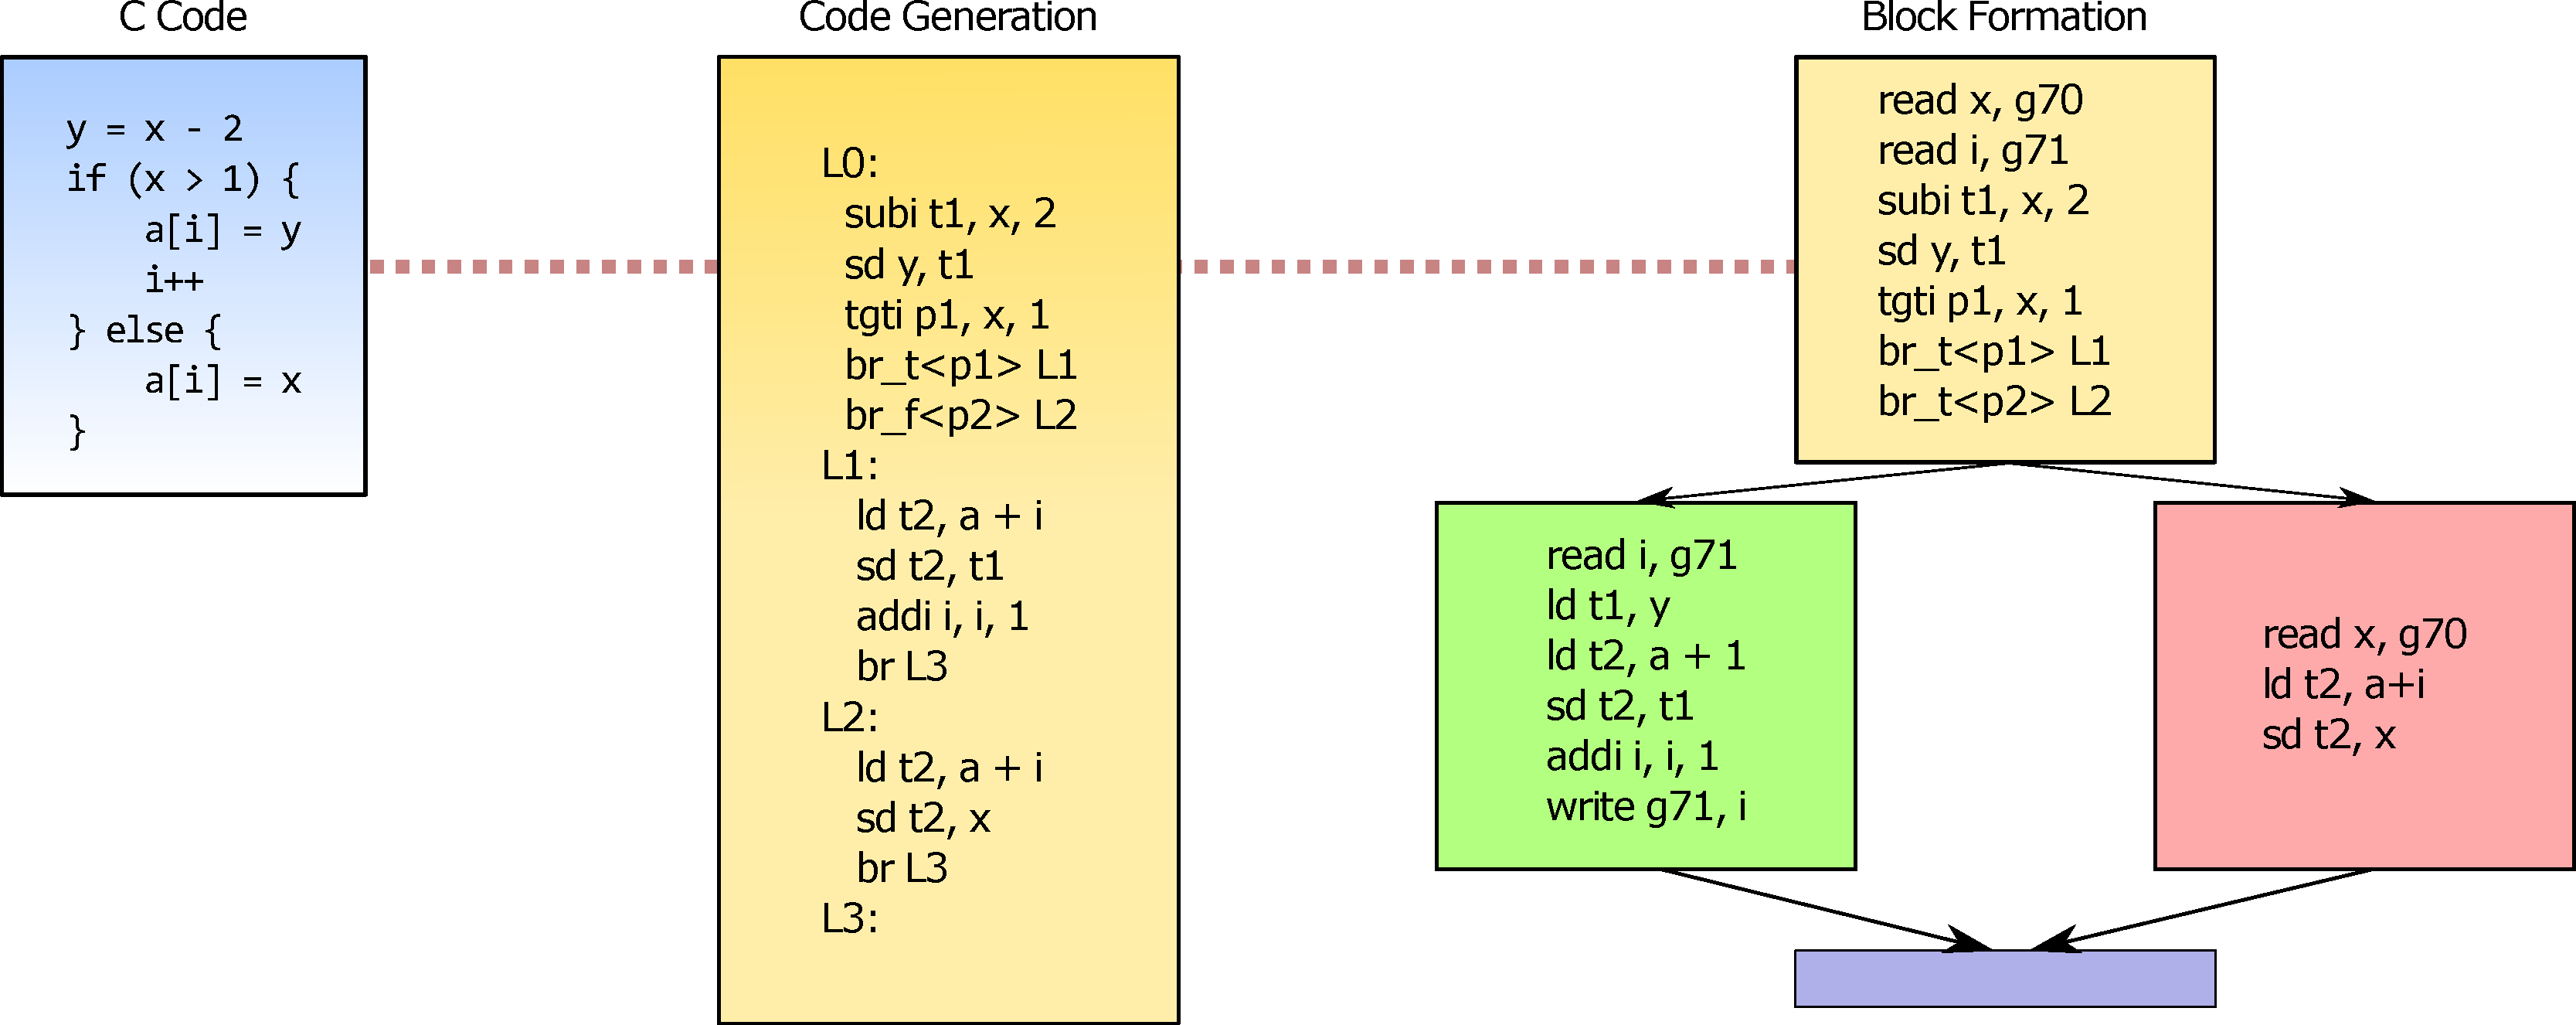
\includegraphics[width=1\textwidth]{background/graphics/EDGE_3.pdf}
    \caption{High-level view of the EDGE ISA flow.}
    \label{fig:EdgeHigh}
\end{figure}

\section{EDGE Instruction Set Architecture} 
The Explicit Data Graph Execution~\cite{burger04edge} (EDGE) instruction set architecture (ISA) is a data-flow based ISA.
Figure~\ref{fig:EdgeHigh} shows a high-level overview of how EDGE differs from a traditional instruction set architecture.
The EDGE compiler has a first pass which generates instructions from the original source code.
Blocks are then generated from the basic-blocks found in the code generation pass.

%what I'm trying to say here is that registers are used only for outer communication, in a block instructions are 
Unlike traditional ISAs, blocks do not communicate via registers, but rather the output targets of instructions are encoded to instruction inputs~\cite{smith2006edge}.
Loads and stores in each EDGE block are assigned unique identifiers which are used resolve load-store dependencies.
Thus, the EDGE ISAs encode dependencies between instructions at the ISA level, registers are only used for inter-communication between blocks.
An EDGE block also contains a header that will inform the hardware about the number of stores and register writes contained in the block~\cite{e2paper}, this is used to facilitate committing blocks.

EDGE blocks also have a set of restrictions to satisfy correctness.
If a block does not meet these requirements, it may need to be broken down into smaller blocks.
These restrictions are:

\begin{itemize}
\item Block Size: an EDGE block may be between 4 to 128 instructions.
\item Load/Store: an EDGE block may have at most 32 load/store instructions.
\item Entry/Exit: an EDGE block may have a single exit but may have multiple exits.
\end{itemize}

To increase the average size of EDGE blocks, multiple blocks can be combined together to form one large block called a hyperblock.
This is achieved through the use of instruction predication.
For example given an if/else statement, the compiler can generate a single block, predicating all instructions of the else statement.
As the compiler needs to declare the number of stores and register writes in the block header, extra instructions may need to be generated to ensure the block always executes the same amount of stores.

Overall, the EDGE ISA enables the architecture to dispatch blocks speculatively, with low overhead~\cite{putnam2010e2,kim2007tflex}, therefore, increasing exploitation of ILP.

\section{EDGE Processor}

\subsection{Core Lanes}
 \begin{figure}[t]
 \center
 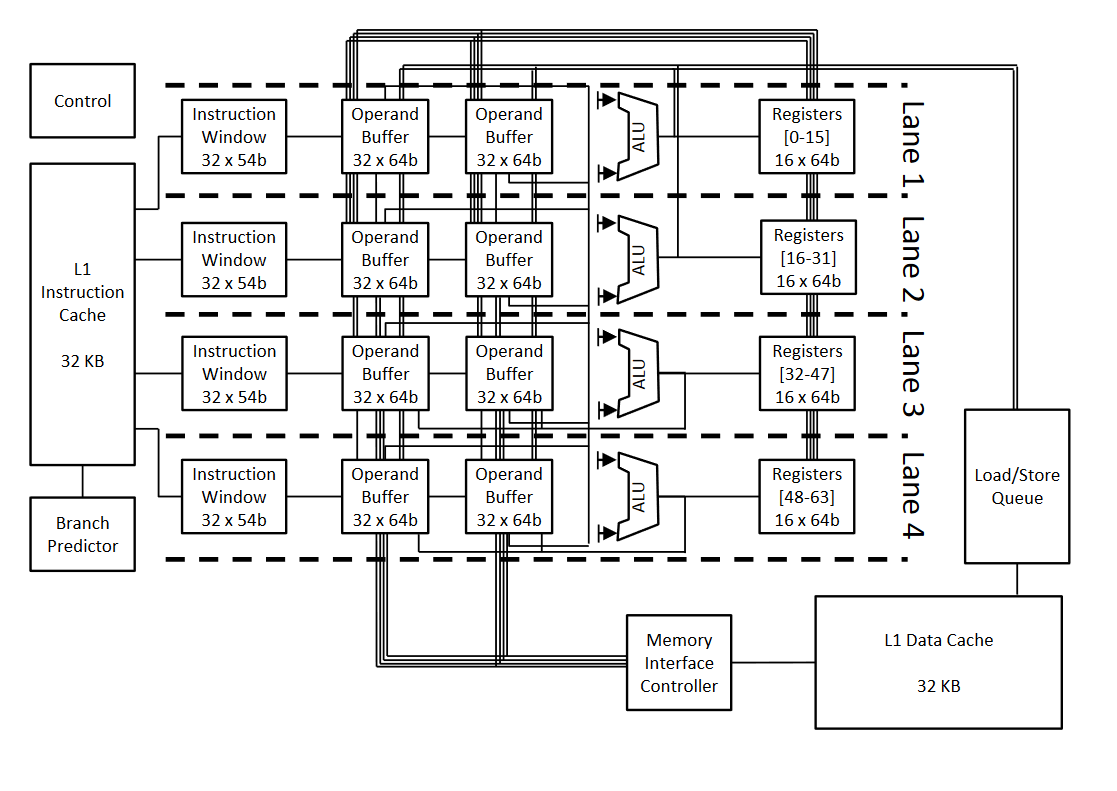
\includegraphics[width=1\textwidth]{background/graphics/e2segment.png}
 \caption{Example of a four lane core on an EDGE processor taken from~\cite{e2smith}.}\label{fig:e2segment}
 \end{figure}
 
EDGE instruction blocks can be up to 128 instructions long, however this often isn't the case.
To maximize core-utilisation, each core on an EDGE Processor is segmented into a set number of lanes which can each fetch and decode their own blocks.
A lane is able to fetch a block of maximum size

\begin{equation}
\frac{128}{NumberOfLanes}
\end{equation}

For example, a four lane core as seen in Figure~\ref{fig:e2segment} can have up to four blocks of 32 instructions.
Fetching blocks larger than 32 instructions will fill up more than one lane.
Depending on the architectural setup, lanes may either share or have their private ALUs.
In case of non-private ALUs, the load-store-queue and register files ensure that memory operations are still happening in order if needed.
Lanes allow EDGE cores to be more flexible to block size variability.

\subsection{Core Fusion}
 \begin{figure}[t]
 \center
 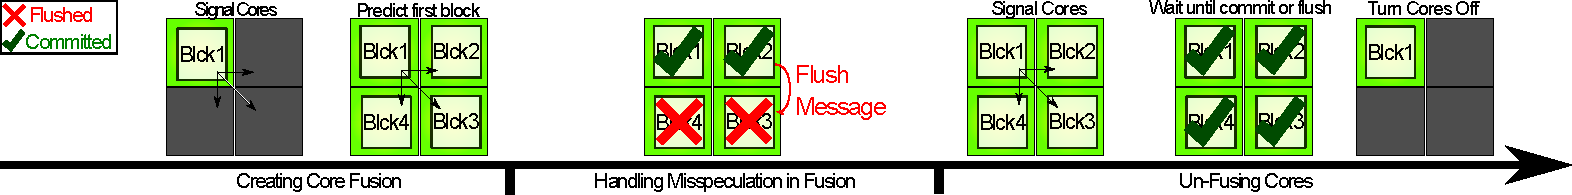
\includegraphics[width=1\textwidth]{cases-paper/graphics/background/proc_test.pdf}
 \caption{Core Fusion Mechanisms for our EDGE-based architecture.}\label{fig:dmp}
 \end{figure}
 
Core Fusion is achieved by fusing a set of \textit{physical} cores to create larger \textit{logical} cores.
This does not modify the physical structure of the chip, instead it provides a unified view of a group of physical cores to the software.
In the processor used throughout the thesis, the micro-architecture is distributed: register files, Load Store Queues (LSQs), L1 caches and ALUs all look like nodes on a network.
This means that when cores fuse together, this is similar to adding an extra node to the network.
Fusion is a dynamic modification and may occur during the execution of a program to better fit the workload.
Unlike traditional CMPs, fused cores will operate on the same thread and attempt to extract Instruction Level Parallelism (ILP) rather than Thread Level Parallelism (TLP)~\cite{micolet2016dmpstream,pricopi2012bahurupi}.

Figure~\ref{fig:dmp} shows the different stages and mechanisms of core fusion for a four core system.
When creating a new core fusion a master core informs all other cores about the fusion and sends the predicted next block address to the next available fused core.
When we start a new thread on a fused core the OS and runtime write the new core mapping to a system register.
The hardware then flushes these cores if they are not idle and sets the PC of the first block of that thread on one core in the logical processor and starts executing.
When a core mispredicts a branch in a fusion, it informs the other cores which flush any younger blocks.
When un-fusing, the master core informs the other cores, which then commit or flush their blocks and power down while the master core continues to fetch and execute blocks from the thread.
The extra hardware required to support dynamic reconfiguration is very minimal~\cite{kim2007tflex} since most of the machinery already in place can be reused such as the cache coherence protocol when fusing and un-fusing the cores.

When a logical core fetches multiple blocks, it may execute them out of order.
However memory instructions and instructions that modify registers pass through the LSQ and register-file and are executed in order.
This ensures that blocks operate on memory in a consistent fashion.
In case of a memory violation caused by undetected dependencies a flush of all blocks younger than the violator, including the violating block, is performed.

%Fusing cores is therefore a lightweight process.
%We estimate that switching the size of the logical-core (LC) results in a delay of 100 cycles on average.
%The actual time varies based on the time it takes the cache coherence protocol to move the data around the memory system.
%Section~\ref{sec:reconfoverhead} discusses in more details how latency affects energy efficiency and shows that dynamic core fusion is still highly beneficial even when considering overheads of 1,000 cycles.

\section{Streaming Programming Languages}

% % This section should explain what steaming programming is (remove all the details about each language)
% General purpose programming languages often propose very little support for programs that handle with a continuous flow of data.
% This results in having to design a set of complicated for loops to manage the streams of data.
% Having to deal with different rates of incoming and outcoming data also increases the complexity of writing these applications using a standard language.

Streaming programming languages are a branch of dataflow programming that focus on applications that deal with a constant stream of data.
These applications, such as audio or video decoding can be commonly found in mobile devices.
Unlike conventional programming languages such as C++, these languages abstract the concept of incoming and outgoing data to permit the programmer to focus on how the data should be treated.
Programs are described as directed graphs where nodes are functions and their edges represent their input and output streams. 
These languages offer primitives to describe such a graph~\cite{theis2002streamit} which expose parallelizable and serial sections of the application directly to the compiler. 
Rates of incoming and outcoming data can also be defined to facilitate load balancing optimizations~\cite{chen2005rawstream}.

Features of streaming programming languages make them an ideal language for targeting multicore processors.
The explicit data communication between the different tasks in the program, the ability to estimate the amount of work performed in each task and information about data rates between tasks allows the compiler to easily generate a multi-threaded application that can run on a dynamic multicore processor.
However, the main challenge consists of deciding how to map the different tasks onto threads and how to allocate the right amount of resources to maximize performance.


\begin{figure}
    \centering
    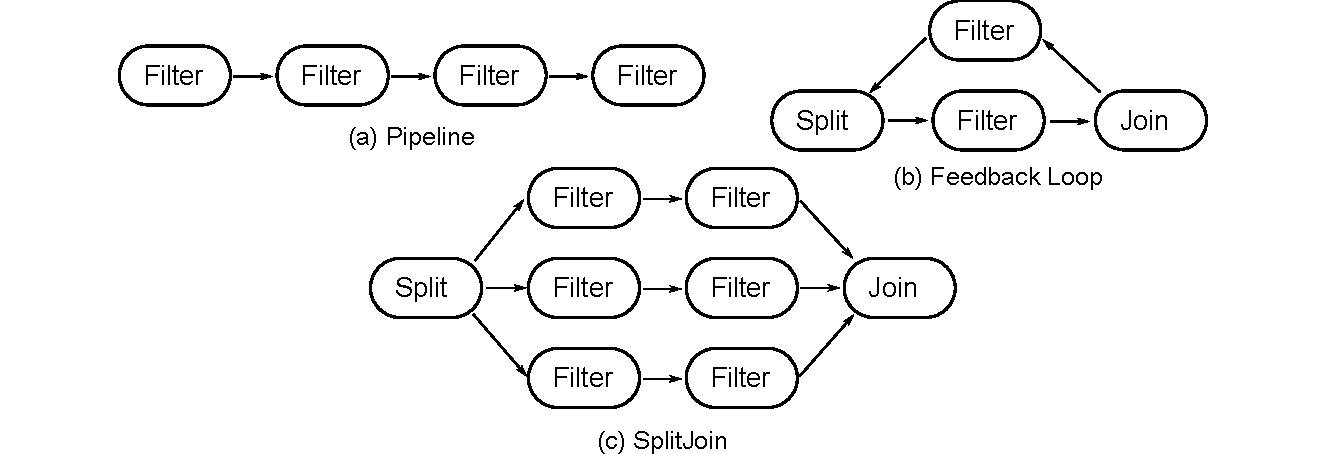
\includegraphics[width=1\textwidth]{streamit-paper/graphics/streamit_types.pdf}
    \caption{Visual representation of the three different StreamIt structures.}
    \label{fig:streamittypes}
\end{figure}

\subsection{StreamIt Programming Language}
StreamIt~\cite{theis2002streamit} is a high-level synchronous dataflow streaming programming language that defines programs as directed graphs.
StreamIt offers an elegant way of describing streaming applications, abstracting away how infinite data streams are managed to allow the programmer to solely focus on how the data must be treated.
A StreamIt program is composed of functions - called \textit{Filters} - which operate on streams of data.
Filters declare a certain amount of data which is to be consumed and produced per schedule.
Filters can be connected via \textit{Pipelines}, \textit{SplitJoins} or \textit{Feedback Loops} to create the streaming application.

Figure~\ref{fig:streamittypes} displays the different methods of connections in detail.
Pipelines (Figure~\ref{fig:streamittypes}(a)) represent a sequence of connecting filters operating on the same stream, each filter in the stream will operate on the output of the previous filter.
In a SplitJoin (Figure~\ref{fig:streamittypes}(c)), data from the stream is passed through a split filter and is either duplicated and passed on in parallel to the filters or distributed amongst the filters in a round-robin fashion.
The output of all the filters in a SplitJoin are then concatenated in a round-robin fashion through a joiner filter.
Finally a Feedback Loop (Figure~\ref{fig:streamittypes}(b)) provides a way for filters to operate on their outputs.
The resulting program written in StreamIt represents a graph where the nodes are filters and their edges represent the incoming and outgoing data streams.

\section{Machine-learning guided optimisations}

Using machine learning to guide optimisations has been a popular area of research as of late~\cite{cummins2017pact,wang2018ml,dubach13dynamic}.
There are two areas in which machine learning is used: compiler driven optimisations and runtime driven optimisations.
Depending on the use, different models will have to be used; for example runtime systems require fast responses, thus the models will have to be smaller, whilst compiler driven optmisations are less pressured by this.

\subsection{Linear Regression}

In a Dynamically reconfigurable processor machine learning can be used to detect when hardware must switch configurations~\cite{micolet2017cases, tavanaElastic}.
Knowing when to reconfigure the processor necessitates fast decision making to minimize the overall cost of reconfiguration.
Machine learning models therefore need to be lightweight to ensure that the computations required to operate the model are as low as possible.
In these situations, a popular model is Linear Regression as it has a fairly low computational footprint~\cite{tavanaElastic}.

Linear Regression assumes a linear relationship between a set of inputs and the predicted output and generates a model in the form of:

\begin{equation}
y = \beta_0 + \beta_1X_1 + \beta_2X_2 + ... + \beta_nX_n
\end{equation}

where y is the predicted output, $X_{1..n}$ are the inputs and $\beta_{0.n}$ are weighted regression coefficients.
When training a linear regression, it generates the $\beta$ weights as to minimize the square-error between the training inputs and predicted outputs.
Once a model has been generated from input data, it can be implemented as a set of sums in hardware, making it an efficient way of making predictions.

\subsection{k Nearest Neighbors}

k Nearest Neighbors can be used for both regression and classification.
In both situations an output is generated by averaging the \textit{k} nearest neighbors to the input from the training data.
The average is often obtained by a weighted sum of the features of the k neighbors.